\documentclass[aspectratio=169]{beamer}

% Custom theme and packages
\usepackage{beamertheme-custom}
% Custom symbols and commands
\usepackage{symbols-custom}

% Specific packages for this lecture if needed
% \usetikzlibrary{...}

\title{Hierarchical (a.k.a.~Multilevel) Modeling}
\author{Joachim Vandekerckhove}
\date{Spring 2025}

\begin{document}

\maketitle

\begin{frame}{Hierarchical modeling}
    A statistical framework for data with \textbf{dependencies} from \textbf{group structure}.
    \pause
    \begin{itemize}
        \item Examples: Students in classrooms, patients in hospitals, trials within participants, stimuli within conditions.
        \item Observations within the same group are typically correlated (non-independent).
        \item Standard methods ignore this structure, which can lead to biased estimates and incorrect inferences.
    \end{itemize}
\end{frame}

\begin{frame}{Pooling is a spectrum}
    \begin{columns}[T] % Align tops
        \begin{column}{0.5\textwidth}
            \textbf{Complete pooling} (ignore structure)\\
            \small Analyze all data together.
            \begin{itemize}
                \item[$\times$] Underestimates errors.
                \item[$\times$] Hides true group differences.
                \item[$\times$] Doesn\'t quantify group variability.
                \item[$\times$] Unlikely to generalize.
            \end{itemize}
        \end{column}
        \begin{column}{0.5\textwidth}
            \textbf{No pooling} (separate analyses)\\
            \small Analyze each group separately.
            \begin{itemize}
                \item[$\times$] Ignores within-group similarities.
                \item[$\times$] Inefficient.
                \item[$\times$] Noisy estimates.
                \item[$\times$] Impossible to generalize.
            \end{itemize}
        \end{column}
    \end{columns}
\end{frame}

\begin{frame}{The compromise: Partial pooling}
    Hierarchical models provide a statistically principled compromise with \textit{partial pooling}.
    
    \pause
    \begin{itemize}
        \item Information is \emph{adaptively shared} across units within populations.
        \pause
        \item Each unit contributes, weighted by its precision.
        \pause
        \item \emph{``Borrow strength''}: Units within populations inform each other.
        \pause
        \item Improves individual unit estimates (especially for noisy/small units) with good prior knowledge.
        \pause
        \item Simultaneously estimates population-level effects \emph{and} the extent of variation between participants.
    \end{itemize}
\end{frame}

\begin{frame}[fragile]{Hierarchical model formulation}
    Let $y_{i|j}$ be outcome for observation $i$ in group $j$, $x_{i|j}$ a predictor.
    \pause

    \begin{itemize}
        \item \textbf{Level 1 (within-group):}
        \\[1ex]
          $ \qquad y_{i|j} = \alpha_j + \beta x_{i|j} + \epsilon_{i|j}$, with $\epsilon_{i|j} \sim \mathcal{N}(0, \sigma^2_y)$
        \\[1ex]
          Intercept $\alpha_j$ varies by participant, while slope $\beta$ is fixed (common).
        \pause
        \item \textbf{Level 2 (between-group):}
        \\[1ex]
          $ \qquad \alpha_j \sim \mathcal{N}(\mu_{\alpha}, \sigma^2_{\alpha}) $
        \\[1ex]
          The group intercepts ($\alpha_j$) are drawn from a population distribution.
        \\[1ex]
          \begin{itemize}
            \item $\mu_{\alpha}$: Population average intercept.
            \item $\sigma^2_{\alpha}$: Variance of intercepts across participants.
          \end{itemize}
    \end{itemize}
    \pause
    \vfill
    This structure explicitly models the dependency within populations.
\end{frame}

\begin{frame}{Hierarchical model structure}
    \begin{figure}
        \centering
        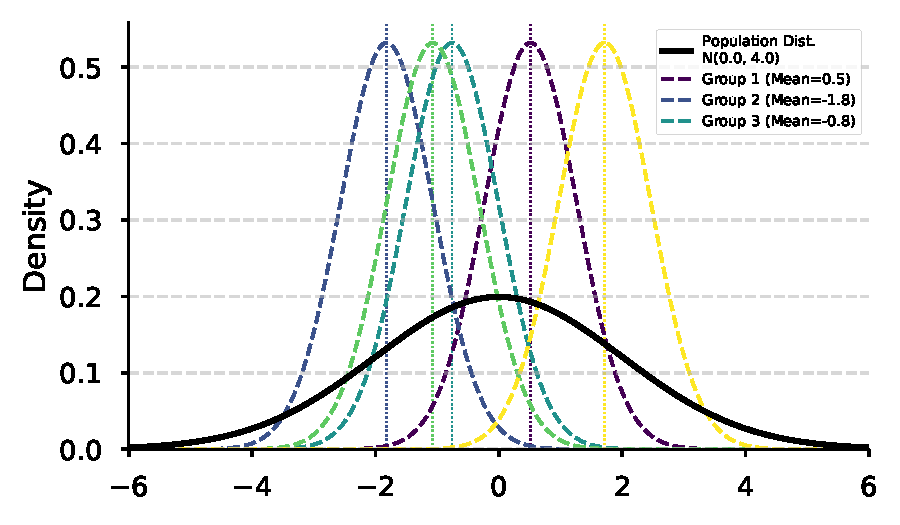
\includegraphics[width=0.65\textwidth]{figures/fig_003_multilevel.pdf}
        \caption{The population distribution (solid black line, representing $N(\mu_{\alpha}, \sigma^2_{\alpha})$) describes the overall tendency for participant means. Person-specific distributions (dashed colored lines, representing $N(\alpha_j, \sigma^2_y)$ for different $j$) have means ($\alpha_j$, marked by dotted vertical lines) drawn from the population distribution.}
    \end{figure}
\end{frame}

\begin{frame}[fragile]{Hierarchical model formulation}
    Let $y_{i|j}$ be outcome for observation $i$ in group $j$, $x_{i|j}$ a predictor.

    \begin{itemize}
        \item[]
          $ \qquad y_{i|j} = \alpha_j + \beta x_{i|j} + \epsilon_{i|j}$, with $\epsilon_{i|j} \sim \mathcal{N}(0, \sigma^2_y)$
        \item[]
          $ \qquad \alpha_j = \mu_{\alpha} + u_j$, with $u_j \sim \mathcal{N}(0, \sigma^2_{\alpha})$
    \end{itemize}

    All together: $y_{i|j} = \mu_{\alpha} + \beta x_{i|j} + u_j + \epsilon_{i|j} $

    This model has a global intercept ($\mu_{\alpha}$), a global slope ($\beta$), a participant-specific deviation ($u_j$), and a residual error ($\epsilon_{i|j}$).
\end{frame}

\begin{frame}{Terminology}
    \begin{itemize}
        \item \textbf{Fixed effects}\\ Parameters that differ between participants and are estimated independently from one another -- they do not share free parameters: $\alpha_1 \sim \mathcal{N}(0, 1), \alpha_2 \sim \mathcal{N}(0, 1), \ldots$
        \pause
        \item \textbf{Random effects}\\ Parameters that differ between participants but are estimated as an interconnected set -- they are affected by shared parameters: $\alpha_1 \sim \mathcal{N}(\mu_{\alpha}, \sigma^2_{\alpha}), \alpha_2 \sim \mathcal{N}(\mu_{\alpha}, \sigma^2_{\alpha}), \ldots$
        \pause
        \item \textbf{Variance components}\\ Parameters characterizing variability at different levels:
        \begin{itemize}
            \item Level 1: Residual variance $\sigma^2_y$.
            \item Level 2: Random effect variances ($\sigma^2_{\alpha}$) quantify the magnitude of inter-individual differences.
        \end{itemize}
    \end{itemize}
\end{frame}

\begin{frame}{Fixed vs.\ random effects}
    \begin{figure}
        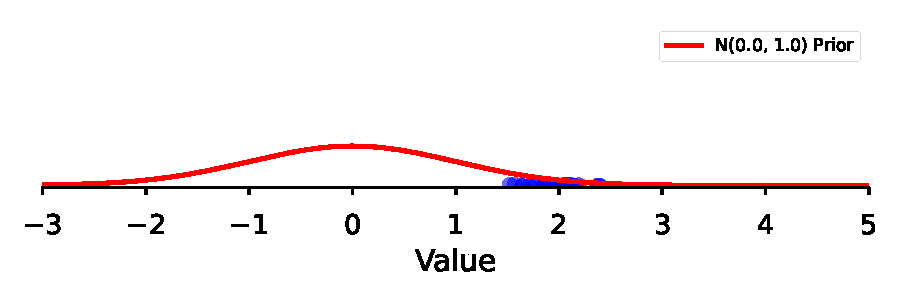
\includegraphics[height=0.45\textheight]{figures/fig_003_prior.pdf}
        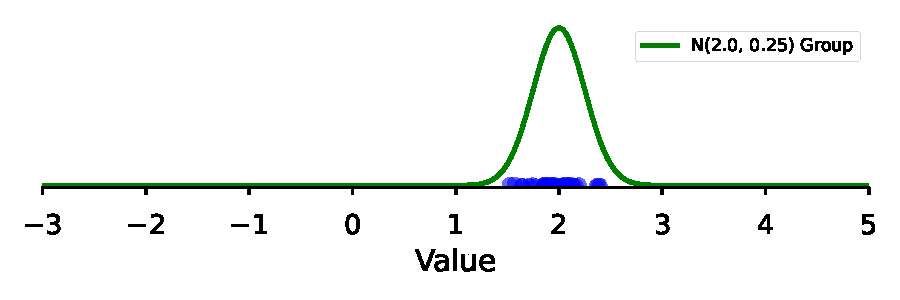
\includegraphics[height=0.45\textheight]{figures/fig_003_partial.pdf}
    \end{figure}
\end{frame}

\begin{frame}{Partial pooling and shrinkage}
    Estimates for person-specific parameters (e.g., $\hat{\alpha}_j$) balance two sources of information:
    \pause
    \begin{enumerate}
        \item From the person's own data (the \emph{no-pooling estimate}, $\hat{\alpha}_{j, \text{no pool}}$).
        \item From the overall population distribution (the \emph{population mean estimate}, $\hat{\mu}_{\alpha}$).
    \end{enumerate}
    \pause
    $$\hat{\alpha}_j \approx w_j \hat{\alpha}_{j, \text{no pool}} + (1-w_j) \hat{\mu}_{\alpha} $$
    \pause
    The weight $w_j$ (or shrinkage factor) depends on precision:\\
    \pause
    $$ w_j \approx \frac{\text{individual precision}}{\text{population precision} + \text{individual precision}} = \frac{1 / \text{Var}(\hat{\alpha}_{j, \text{no pool}})}{1 / \text{Var}(\hat{\alpha}_{j, \text{no pool}}) + 1 / \sigma^2_{\alpha}} $$
    \pause
    $\text{Var}(\hat{\alpha}_{j, \text{no pool}})$ depends on participant sample size $n_j$ and within-participant variance $\sigma^2_y$.
    Person-specific estimates are \textbf{shrunk} towards the population mean.
\end{frame}

\begin{frame}{Adaptive shrinkage}
    The amount of shrinkage is automatically \emph{adaptive} and data-dependent:

    \textbf{More shrinkage} (towards $\hat{\mu}_{\alpha}$) when:
    \begin{itemize}
        \item Participant has \emph{less data} / noisy estimate (large $\text{Var}(\hat{\alpha}_{j, \text{no pool}})$).
        \item Participants are very \emph{similar} (small between-participant variance $\sigma^2_{\alpha}$).
    \end{itemize}
    \pause
    \medskip
    \textbf{Less shrinkage} (estimate closer to participant's own data) when:
    \begin{itemize}
        \item Participant has \emph{more data} / precise estimate (small $\text{Var}(\hat{\alpha}_{j, \text{no pool}})$).
        \item Participants are very \emph{dissimilar} (large between-participant variance $\sigma^2_{\alpha}$).
    \end{itemize}
\end{frame}

\begin{frame}{Shrinkage visualization}
    \begin{figure}
        \centering
        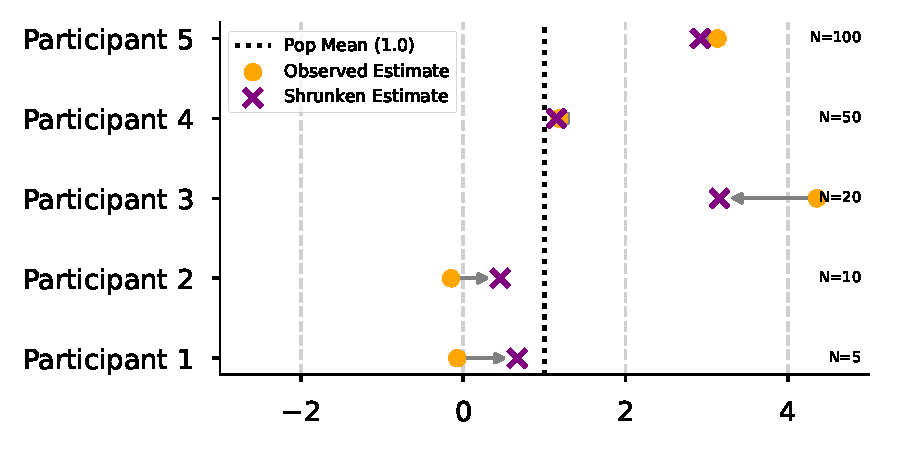
\includegraphics[width=0.7\textwidth]{figures/fig_003_shrinkage.pdf}
        \caption{Observed group means (\textcolor{orange}{o}) are pulled towards the estimated population mean (dashed line). The amount of shrinkage (length of gray arrow) is greater for groups with less data (smaller $n_j$), resulting in the shrunken estimates (\textcolor{purple}{x}). The overall population mean estimate itself is informed by all participants.}
    \end{figure}
\end{frame}

\begin{frame}[fragile]{Bayesian implementation}
    Bayesian methods provide a natural framework:
    \pause
    \begin{itemize}
        \item \textbf{Full probability model:} Specify the entire structure:
        \begin{itemize}
            \item Level 1 likelihood: $P(\text{Data} | \text{Level 1 Params})$
            \item Level 2 priors: $P(\text{Level 1 Params} | \text{Level 2 Hyperparams})$
            \item Hyperpriors: $P(\text{Level 2 Hyperparams})$
        \end{itemize}
        \pause
        \item \textbf{Coherent uncertainty:} Get full posterior distributions for \emph{all} parameters (fixed effects, random effects, variance components), naturally propagating uncertainty.
        \pause
        \item \textbf{Computation:} Modern MCMC (e.g., HMC/NUTS in Stan, PyMC) handles complex posteriors effectively.
        \pause
        \item \textbf{Prior specification:} Requires care!
        \begin{itemize}
            \item Fixed Effects / Means ($\mu$s): Often weakly informative (e.g., wide Normal).
            \item Variance Components ($\sigma$s): Crucial! Use weakly informative priors concentrated away from zero (e.g., Half-Normal, Half-Cauchy) to avoid issues.
        \end{itemize}
    \end{itemize}
\end{frame}

\begin{frame}[fragile]{Model checking and interpretation}
    Fitting is just the start! Rigorous checking is essential:
    \pause
    \begin{itemize}
        \item \textbf{MCMC convergence:} Check $\hat{R}$ (should be $\approx 1.0$), Effective Sample Size (ESS), trace plots.
        \pause
        \item \textbf{Prior sensitivity analysis:} Do results change much with different reasonable priors?
        \pause
        \item \textbf{Posterior predictive checks (PPCs):}
        \begin{itemize}
            \item Simulate data from the fitted model.
            \item Compare simulated data distributions to observed data. Mismatches indicate model problems.
        \end{itemize}
    \end{itemize}
    \pause
    \vfill
    \textbf{Interpretation:} Focus on population parameters ($\mu$s, fixed $\beta$s), magnitude of variation ($\sigma$s), and potentially shrunken group estimates ($\alpha_j$s, $\beta_j$s), always with uncertainty (posterior distributions / intervals).
\end{frame}

\begin{frame}[fragile]{Crossed vs.\ nested random effects}
    \begin{itemize}
        \item Nested: Students in classrooms, classrooms in schools.
        $$y_{i|c|s} = \alpha_{c|s} + \beta x_{i|c,s} + \gamma_{s} + \epsilon_{i|c,s}$$
        \item Crossed: Participants respond to multiple stimuli (random effects for participant AND stimulus, not nested).
        $$y_{ip} = \alpha_{p} + \gamma_{i} + \epsilon_{ip}$$
    \end{itemize}
\end{frame}

\begin{frame}[fragile]{Parameter identification}
    \begin{itemize}
        \item Identification: There exists a unique solution for the parameters given the data.\pause
        \item Sometimes you can accidentally build a non-identified model.\pause
        \item Here is a common example:
        $$
            y_{ip} = \alpha_{p} + \gamma_{i} + \epsilon_{ip} \text{ ~with~ } \begin{cases}
                \alpha_{p} \sim \text{N}(\mu_{\alpha}, \sigma^2_{\alpha}) \\
                \gamma_{i} \sim \text{N}(\mu_{\gamma}, \sigma^2_{\gamma})
            \end{cases}
        $$
        \item If I increase $\mu_{\alpha}$ by $x$ and decrease $\mu_{\gamma}$ by $x$, the model makes identical predictions.
        \item This is a non-identified model.\pause
        \item Fitting the model will go poorly -- if there aren't convergence issues, you will see that the posterior distributions for $\mu_{\alpha}$ and $\mu_{\gamma}$ are strongly negatively correlated.\pause
        \item The solution is to add a \emph{constraint}, for example $\mu_{\alpha} = 0$.
    \end{itemize}
\end{frame}

\begin{frame}[fragile]{Generalization to cognitive modeling}
    \begin{eqnarray*}
        y_{ip} &=& \alpha_{p} + \gamma_{i} + \epsilon_{ip} \text{ ~with~ } \epsilon_{ip} \sim {N}(0, \sigma^2_{ip})\\
        \Leftrightarrow \quad
        y_{ip} &\sim& {N}(\alpha_{p} + \gamma_{i}, \sigma^2_{ip})
    \end{eqnarray*}

    In cognitive modeling, data are rarely normally distributed.
    
    How do we deal with this?
\end{frame}

\begin{frame}[fragile]{Lessons from psychometrics}
    \begin{itemize}
        \item In psychometrics, we deal with binary data (e.g., correct/incorrect responses).
        \pause
        \item A useful distribution for this is the \textbf{Bernoulli distribution}:
        $$y_{ip} \sim \text{Bernoulli}(\pi_{ip})$$
        \pause
        \item Now we handle the \emph{Bernoulli parameter} as a to-be-explained dependent variable:
        $$ \pi_{ip} = \alpha_{p} + \gamma_{i} \quad \Leftrightarrow \quad \pi_{ip} \sim \text{Bernoulli}(\alpha_{p} + \gamma_{i}) $$
        \pause
        \item Psychometricians refer to $\alpha_{p}$ as the \emph{person side} and $\gamma_{i}$ as the \emph{item side}.
        \pause
        \item We can also handle either of these as a to-be-explained dependent variable:
        $$ \alpha_{p} = \beta_0 + \beta_1 z_p + \ldots$$
        $$ \gamma_{i} = \zeta_0 + \zeta_1 q_i + \ldots$$
    \end{itemize}
\end{frame}

\begin{frame}[fragile]{See the pattern}
    First, in linear models (with normally distributed data), we did this decomposition:
    $$y_{ip} \sim {N}(\mu_{ip}, \sigma^2_{ip}) \quad \Leftrightarrow \quad y_{ip} \sim N(\alpha_{p} + \gamma_{i}, \sigma^2_{ip})$$
    \pause
    Then, in psychometrics (with binary data), we did this decomposition:
    $$y_{ip} \sim \text{Bernoulli}(\pi_{ip}) \quad \Leftrightarrow \quad y_{ip} \sim \text{Bernoulli}(\alpha_{p} + \gamma_{i})$$
    \pause
    Now, in cognitive modeling (with complex distributions), we're going to do this:
    $$y_{ip} \sim \text{Cognitive}(\psi_{ip}, \varsigma_{ip}) \quad \Leftrightarrow \quad y_{ip} \sim \text{Cognitive}(\alpha_{p} + \gamma_{i}, \varsigma_{ip})$$
    \pause
    As we go, we'll declare some parameters to be focal ($\psi_{ip}$) and others nuisance ($\varsigma_{ip}$).
\end{frame}

\begin{frame}[fragile]{Hierarchical cognitive models}

    This is just one way of decomposing model parameters:

    $$y_{ip} \sim \text{Cognitive}(\psi_{ip}, \varsigma_{ip}) \quad \Leftrightarrow \quad y_{ip} \sim \text{Cognitive}(\alpha_{p} + \gamma_{i}, \varsigma_{ip})$$

    Having a hierarchical structure is optional, but almost always the right call:

    $$\alpha_{p} \sim \text{N}(\mu_{\alpha}, \sigma^2_{\alpha})$$

    Maybe $\mu_{\alpha} = \beta_0 + \beta_1 z_p + \ldots$ really the world is your oyster at this point.

\end{frame}

\begin{frame}[fragile]{Putting it all together}

    We can now write a hierarchical model for any cognitive model.\pause

    Say $y_{ip}$ is person $p$'s data from condition $i$: \pause \emph{$y_{ip} = \left(\text{hit rate}_{ip}, \text{false alarm rate}_{ip}\right)$}\pause
    \begin{eqnarray*}
        y_{ip} &\sim& \text{SDT}(d'_{ip}, c'_{ip}) \\
        d'_{ip} &=& \alpha_{p} + \gamma_{i} \\
        \gamma_{i} &=& \zeta_{0} + \zeta_{1} \text{brightness}_{i} \\
        \alpha_{p} &\sim& \text{N}(\mu_{\alpha}, \sigma^2_{\alpha})
    \end{eqnarray*}
    ... where $\text{SDT}\left(\right)$ is shorthand for the signal detection theory functions covered earlier.
    \pause

    The rest is just a lot of typing.\pause

    This is an unidentified model, can you see why?
\end{frame}

\begin{frame}[fragile]{Assignment: Constrain an SDT model}
    Change how sensitivity ($d'$) is modeled across conditions ($k$) in \texttt{conditional.py}.

    \begin{columns}[T] % Align tops
        \begin{column}{0.45\textwidth}
            \textbf{Currently: conditional SDT model} \\
            \begin{itemize}
                \item Independent $d'$ per condition
                \item $d'_{k} \sim \mathcal{N}(0, 2^2)$
                \item Estimates an independent $d'_k$ for each condition $k$
                \item Uses three free parameters to model $d'_k$
            \end{itemize}
        \end{column}

        \begin{column}{0.6\textwidth}
            \textbf{Desired: Condition \emph{explanatory} SDT model} \\
            \begin{itemize}
                \item Linear effect of difficulty $C_k$ on $d'_k$
                \item $d'_k = \beta_0 + \beta_1 \times C_k$, with
                \begin{itemize}
                \item $C=-1$ for `Easy'
                \item $C=0$ for `Medium'
                \item $C=1$ for `Hard'
                \end{itemize}
                \item Uses only two free parameters to model $d'_k$:
                \begin{itemize}
                    \item $\beta_0 \sim \mathcal{N}(0, 2^2)$
                    \item $\beta_1 \sim \mathcal{N}(0, 0.5^2)$
                \end{itemize}
                \item Estimates intercept and slope; $d'_k$ is derived.
            \end{itemize}
        \end{column}
    \end{columns}
\end{frame}

\begin{frame}[fragile]{Advanced assignment: Constrain a hierarchical SDT model}
    Change how group-level sensitivity ($d'$) is modeled across conditions ($k$) in \texttt{full.py}.
    
    In either case, at the individual level, parameters for person $p$ in condition $k$ come from a population distribution: $d'_{pk} \sim \mathcal{N}(\mu_{k}, \sigma_{k}^2)$, with $\sigma_{k} \sim \text{HalfNormal}(1)$.\\[3ex]

    \begin{columns}[T] % Align tops
        \begin{column}{0.5\textwidth}
            \textbf{Current full hierarchical model} \\
            \begin{itemize}
            \item The parameters of the population distribution are independent per condition:
            \begin{itemize}
                \item $\mu_{k} \sim \mathcal{N}(0, 2^2)$
            \end{itemize}
            \item Estimates a separate mean $\mu_{k}$ for each condition.
            \end{itemize}
        \end{column}

        \begin{column}{0.55\textwidth}
            \textbf{Condition explanatory hierarchical model} \\
            \begin{itemize}
            \item The mean of the $d'$ population distribution is linear over conditions:
            \begin{itemize}
                \item $\mu_{k} = \beta_0 + \beta_1 \times C_k$
            \end{itemize}
            \item[] with
                \begin{itemize}
                    \item $\beta_0 \sim \mathcal{N}(0, 2^2)$
                    \item $\beta_1 \sim \mathcal{N}(0, 0.5^2)$
                \end{itemize}
            \end{itemize}
            Estimates intercept and slope; $\mu_{k}$ is derived.
        \end{column}
    \end{columns}
\end{frame}

\maketitle

\end{document} 